\documentclass[
11pt, % Set the default font size, options include: 8pt, 9pt, 10pt, 11pt, 12pt, 14pt, 17pt, 20pt
%t, % Uncomment to vertically align all slide content to the top of the slide, rather than the default centered
%aspectratio=169, % Uncomment to set the aspect ratio to a 16:9 ratio which matches the aspect ratio of 1080p and 4K screens and projectors
]{beamer}

\graphicspath{{Images/}{./}} % Specifies where to look for included images (trailing slash required)

\usepackage{todonotes}
\usepackage{graphicx}
\usepackage{xcolor}
\usepackage{subfig}
%%\usepackage[noend]{algpseudocode}


\usepackage{algorithm}
\usepackage{algorithmic}

\usepackage{blkarray}
\usepackage{amsmath}
\usepackage{xspace}
\usepackage{float}


\usepackage{tikz}
\usetikzlibrary{matrix, decorations, patterns, positioning, shapes, calc, intersections, arrows, fit}

\usetikzlibrary{patterns}
\usetikzlibrary{fit,calc,positioning,decorations.pathreplacing,matrix,3d, hobby}

\usepackage{booktabs} % Allows the use of \toprule, \midrule and \bottomrule for better rules in tables


\newcommand{\brown}[1]{{\color{brown} #1 }}

%% Colors from https://latexcolor.com/
\definecolor{pastelviolet}{rgb}{0.8, 0.6, 0.79}
\definecolor{babyblueeyes}{rgb}{0.63, 0.79, 0.95}
\definecolor{pastelyellow}{rgb}{0.99, 0.99, 0.59}
\definecolor{pastelgreen}{rgb}{0.47, 0.87, 0.47}
\definecolor{pastelred}{rgb}{1.0, 0.41, 0.38}
\colorlet{patternblue}{blue!60}


\colorlet{darkred}{red!80!black}
\colorlet{darkblue}{blue!80!black}
\newcommand<>{\darkred}[1]{{\color{darkred}{#1}}}
\newcommand<>{\darkblue}[1]{{\color#2{blue!50!black!100}{#1}}}

\usetheme{Madrid}





%----------------------------------------------------------------------------------------
%	PRESENTATION INFORMATION
%----------------------------------------------------------------------------------------

\title[collective communication]{Collective communication costs in MPI} % The short title in the optional parameter appears at the bottom of every slide, the full title in the main parameter is only on the title page

%\subtitle{Optional Subtitle} % Presentation subtitle, remove this command if a subtitle isn't required

\author[Suraj Kumar]{Suraj Kumar} % Presenter name(s), the optional parameter can contain a shortened version to appear on the bottom of every slide, while the main parameter will appear on the title slide

\institute[Inria \& ENS Lyon]{Inria \& ENS Lyon \\ \smallskip Email:\textit{suraj.kumar@inria.fr}} % Your institution, the optional parameter can be used for the institution shorthand and will appear on the bottom of every slide after author names, while the required parameter is used on the title slide and can include your email address or additional information on separate lines

\date[CR12]{CR12: September 2023\\ \smallskip\small https://surakuma.github.io/courses/daamtc.html} % Presentation date or conference/meeting name, the optional parameter can contain a shortened version to appear on the bottom of every slide, while the required parameter value is output to the title slide

%----------------------------------------------------------------------------------------

\begin{document}
	
	%----------------------------------------------------------------------------------------
	%	TITLE SLIDE
	%----------------------------------------------------------------------------------------
	
	\begin{frame}
		\titlepage % Output the title slide, automatically created using the text entered in the PRESENTATION INFORMATION block above
	\end{frame}


\begin{frame}{Cost model}
	\begin{itemize}
		\item The links of the network are bidirectional
		\item Each process can send and receive one message at the same time
		\item Time taken to send a message with $n$ bytes between any two nodes --  $T= \alpha + n\beta$
		\begin{itemize}
			\item $\alpha$: latency cost per message, $\beta$: transfer time per byte
		\end{itemize}
		\item In case of reduction operation, $\gamma$: computation cost per byte 		
	\end{itemize}
\end{frame}

\begin{frame}{Allgather}
\begin{minipage}{0.45\linewidth}
	\begin{center}
		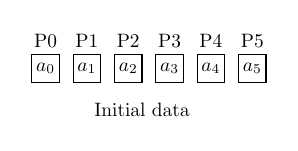
\begin{tikzpicture}[scale=0.35, every node/.style={transform shape}]
		
		%//starting at (0,0)
		
		\foreach \x in {0,1,2,3,4, 5}
		{
		\draw (1.5*\x, 0) -- ++(1, 0) -- ++(0,1) -- ++(-1,0) -- cycle;
		\node [scale=2] at (1.5*\x+0.5, 0.5) {$a_\x$};
		}
		
		
		\foreach \x in {0,1,2,3,4, 5}
		\node [scale=2] at (1.5*\x+0.5 , 1.5) {P\x};
		
		\node [scale=2] at (4, -1) {$\textnormal{Initial data}$};
		\end{tikzpicture}
			
	\end{center}
\end{minipage}
\begin{minipage}{0.45\linewidth}
	\begin{center}
			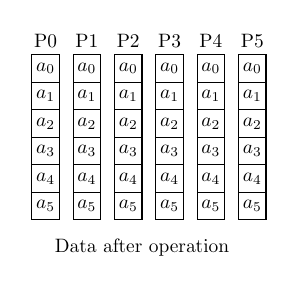
\begin{tikzpicture}[scale=0.35, every node/.style={transform shape}]
		
		%//starting at (0,0)
		
		\draw (0,0) -- (0,6) -- (1,6) -- (1,0) -- cycle;
		\foreach \x in {0,1,2,3,4, 5, 6}
		\draw (0,\x) -- (1,\x);
		
		\foreach \x/\val in {0/$a_5$,1/$a_4$,2/$a_3$,3/$a_2$,4/$a_1$, 5/$a_0$}
		\node [scale=2] at (0.5, 0.5 + \x) {\val};
		
		\foreach \x in {0,1,2,3,4, 5}
		\node [scale=2] at (1.5*\x+0.5 , 6.5) {P\x};
		
		\def\xstep{1.5}
		
		\draw (\xstep+0,0) -- (\xstep+0,6) -- (\xstep+1,6) -- (\xstep+1,0) -- cycle;
		\foreach \x in {0,1,2,3,4, 5, 6}
		\draw (\xstep+0,\x) -- (\xstep+1,\x);
		
		\foreach \x/\val in {0/$a_5$,1/$a_4$,2/$a_3$,3/$a_2$,4/$a_1$, 5/$a_0$}
		\node [scale=2] at (\xstep+0.5, 0.5 + \x) {\val};
		
		\def\xstep{3}
		
		\draw (\xstep+0,0) -- (\xstep+0,6) -- (\xstep+1,6) -- (\xstep+1,0) -- cycle;
		\foreach \x in {0,1,2,3,4, 5, 6}
		\draw (\xstep+0,\x) -- (\xstep+1,\x);
		
		\foreach \x/\val in {0/$a_5$,1/$a_4$,2/$a_3$,3/$a_2$,4/$a_1$, 5/$a_0$}
		\node [scale=2] at (\xstep+0.5, 0.5 + \x) {\val};
		
		
		\def\xstep{4.5}
		
		\draw (\xstep+0,0) -- (\xstep+0,6) -- (\xstep+1,6) -- (\xstep+1,0) -- cycle;
		\foreach \x in {0,1,2,3,4, 5, 6}
		\draw (\xstep+0,\x) -- (\xstep+1,\x);
		
		\foreach \x/\val in {0/$a_5$,1/$a_4$,2/$a_3$,3/$a_2$,4/$a_1$, 5/$a_0$}
		\node [scale=2] at (\xstep+0.5, 0.5 + \x) {\val};
		
		\def\xstep{6}
		
		\draw (\xstep+0,0) -- (\xstep+0,6) -- (\xstep+1,6) -- (\xstep+1,0) -- cycle;
		\foreach \x in {0,1,2,3,4, 5, 6}
		\draw (\xstep+0,\x) -- (\xstep+1,\x);
		
		\foreach \x/\val in {0/$a_5$,1/$a_4$,2/$a_3$,3/$a_2$,4/$a_1$, 5/$a_0$}
		\node [scale=2] at (\xstep+0.5, 0.5 + \x) {\val};
		
		\def\xstep{7.5}
		
		\draw (\xstep+0,0) -- (\xstep+0,6) -- (\xstep+1,6) -- (\xstep+1,0) -- cycle;
		\foreach \x in {0,1,2,3,4, 5, 6}
		\draw (\xstep+0,\x) -- (\xstep+1,\x);
		
		\foreach \x/\val in {0/$a_5$,1/$a_4$,2/$a_3$,3/$a_2$,4/$a_1$, 5/$a_0$}
		\node [scale=2] at (\xstep+0.5, 0.5 + \x) {\val};
		
		\node [scale=2] at (4, -1) {$\textnormal{Data after operation}$};
		\end{tikzpicture}
	\end{center}
\end{minipage}
\vfill
\begin{block}{Ring algorithm (Old agorithm in MPI)}
	\begin{itemize}
		\item Takes total $p-1$ steps
		\item In each step, process $i$ sends its contribution to process $i + 1$ and receives the contribution from process $i- 1$
		\item $T_{ring} = (p-1)\alpha + \left(\frac{p-1}{p}\right)n\beta$
		\item $n$ is the total amount of data gathered on each processor 
	\end{itemize}
\end{block}
\end{frame}
\begin{frame}{Recursive doubling algorithm for Allgather}
	\begin{itemize}
		\item Assume $p$ is a perfect power of $2$
		\item In each step $k(0\le k <\lg p)$, processes that are a distance $2^k$ apart exchange their data
		\item $T_{rec_dbl} = \lg p \alpha + \left(\frac{p-1}{p}\right)n\beta$ 
		\item Working not clear when $p$ is not a-power-of-two  
	\end{itemize}
\end{frame}

\begin{frame}{Bruck's algorithm for Allgather}
	
	
\begin{minipage}{0.3\linewidth}
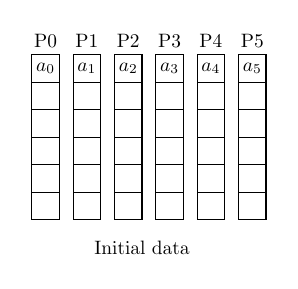
\begin{tikzpicture}[scale=0.35, every node/.style={transform shape}]

%//starting at (0,0)

\draw (0,0) -- (0,6) -- (1,6) -- (1,0) -- cycle;
\foreach \x in {0,1,2,3,4, 5, 6}
\draw (0,\x) -- (1,\x);


\foreach \x in {0,1,2,3,4, 5}
\node [scale=2] at (1.5*\x+0.5 , 6.5) {P\x};

\foreach \x/\val in {0/$ $,1/$ $,2/$ $,3/$ $,4/$ $, 5/$a_0$}
\node [scale=2] at (0.5, 0.5 + \x) {\val};

\def\xstep{1.5}

\draw (\xstep+0,0) -- (\xstep+0,6) -- (\xstep+1,6) -- (\xstep+1,0) -- cycle;
\foreach \x in {0,1,2,3,4, 5, 6}
\draw (\xstep+0,\x) -- (\xstep+1,\x);

\foreach \x/\val in {0/$ $,1/$ $,2/$ $,3/$ $,4/$ $, 5/$a_1$}
\node [scale=2] at (\xstep+0.5, 0.5 + \x) {\val};

\def\xstep{3}

\draw (\xstep+0,0) -- (\xstep+0,6) -- (\xstep+1,6) -- (\xstep+1,0) -- cycle;
\foreach \x in {0,1,2,3,4, 5, 6}
\draw (\xstep+0,\x) -- (\xstep+1,\x);

\foreach \x/\val in {0/$ $,1/$ $,2/$ $,3/$ $,4/$ $, 5/$a_2$}
\node [scale=2] at (\xstep+0.5, 0.5 + \x) {\val};


\def\xstep{4.5}

\draw (\xstep+0,0) -- (\xstep+0,6) -- (\xstep+1,6) -- (\xstep+1,0) -- cycle;
\foreach \x in {0,1,2,3,4, 5, 6}
\draw (\xstep+0,\x) -- (\xstep+1,\x);

\foreach \x/\val in {0/$ $,1/$ $,2/$ $,3/$ $,4/$ $, 5/$a_3$}
\node [scale=2] at (\xstep+0.5, 0.5 + \x) {\val};

\def\xstep{6}

\draw (\xstep+0,0) -- (\xstep+0,6) -- (\xstep+1,6) -- (\xstep+1,0) -- cycle;
\foreach \x in {0,1,2,3,4, 5, 6}
\draw (\xstep+0,\x) -- (\xstep+1,\x);

\foreach \x/\val in {0/$ $,1/$ $,2/$ $,3/$ $,4/$ $, 5/$a_4$}
\node [scale=2] at (\xstep+0.5, 0.5 + \x) {\val};

\def\xstep{7.5}

\draw (\xstep+0,0) -- (\xstep+0,6) -- (\xstep+1,6) -- (\xstep+1,0) -- cycle;
\foreach \x in {0,1,2,3,4, 5, 6}
\draw (\xstep+0,\x) -- (\xstep+1,\x);

\foreach \x/\val in {0/$ $,1/$ $,2/$ $,3/$ $,4/$ $, 5/$a_5$}
\node [scale=2] at (\xstep+0.5, 0.5 + \x) {\val};


\node [scale=2] at (4, -1) {$\textnormal{Initial data}$};
\end{tikzpicture}
\end{minipage}
\begin{minipage}{0.3\linewidth}
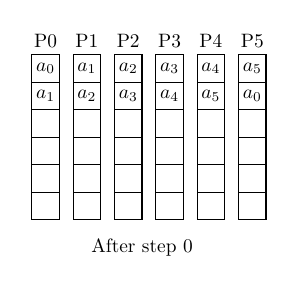
\begin{tikzpicture}[scale=0.35, every node/.style={transform shape}]

%//starting at (0,0)

\draw (0,0) -- (0,6) -- (1,6) -- (1,0) -- cycle;
\foreach \x in {0,1,2,3,4, 5, 6}
\draw (0,\x) -- (1,\x);

\foreach \x/\val in {0/$ $,1/$ $,2/$ $,3/$ $,4/$a_1$, 5/$a_0$}
\node [scale=2] at (0.5, 0.5 + \x) {\val};

\foreach \x in {0,1,2,3,4, 5}
\node [scale=2] at (1.5*\x+0.5 , 6.5) {P\x};

\def\xstep{1.5}

\draw (\xstep+0,0) -- (\xstep+0,6) -- (\xstep+1,6) -- (\xstep+1,0) -- cycle;
\foreach \x in {0,1,2,3,4, 5, 6}
\draw (\xstep+0,\x) -- (\xstep+1,\x);

\foreach \x/\val in {0/$ $,1/$ $,2/$ $,3/$ $,4/$a_2$, 5/$a_1$}
\node [scale=2] at (\xstep+0.5, 0.5 + \x) {\val};

\def\xstep{3}

\draw (\xstep+0,0) -- (\xstep+0,6) -- (\xstep+1,6) -- (\xstep+1,0) -- cycle;
\foreach \x in {0,1,2,3,4, 5, 6}
\draw (\xstep+0,\x) -- (\xstep+1,\x);

\foreach \x/\val in {0/$ $,1/$ $,2/$ $,3/$ $,4/$a_3$, 5/$a_2$}
\node [scale=2] at (\xstep+0.5, 0.5 + \x) {\val};


\def\xstep{4.5}

\draw (\xstep+0,0) -- (\xstep+0,6) -- (\xstep+1,6) -- (\xstep+1,0) -- cycle;
\foreach \x in {0,1,2,3,4, 5, 6}
\draw (\xstep+0,\x) -- (\xstep+1,\x);

\foreach \x/\val in {0/$ $,1/$ $,2/$ $,3/$ $,4/$a_4$, 5/$a_3$}
\node [scale=2] at (\xstep+0.5, 0.5 + \x) {\val};

\def\xstep{6}

\draw (\xstep+0,0) -- (\xstep+0,6) -- (\xstep+1,6) -- (\xstep+1,0) -- cycle;
\foreach \x in {0,1,2,3,4, 5, 6}
\draw (\xstep+0,\x) -- (\xstep+1,\x);

\foreach \x/\val in {0/$ $,1/$ $,2/$ $,3/$ $,4/$a_5$, 5/$a_4$}
\node [scale=2] at (\xstep+0.5, 0.5 + \x) {\val};

\def\xstep{7.5}

\draw (\xstep+0,0) -- (\xstep+0,6) -- (\xstep+1,6) -- (\xstep+1,0) -- cycle;
\foreach \x in {0,1,2,3,4, 5, 6}
\draw (\xstep+0,\x) -- (\xstep+1,\x);

\foreach \x/\val in {0/$ $,1/$ $,2/$ $,3/$ $,4/$a_0$, 5/$a_5$}
\node [scale=2] at (\xstep+0.5, 0.5 + \x) {\val};


\node [scale=2] at (4, -1) {$\textnormal{After step $0$}$};
\end{tikzpicture}
\end{minipage}
\begin{minipage}{0.3\linewidth}
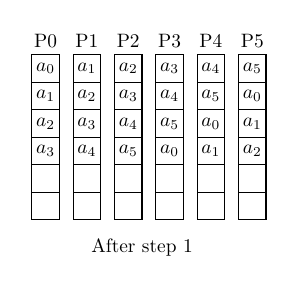
\begin{tikzpicture}[scale=0.35, every node/.style={transform shape}]

%//starting at (0,0)

\draw (0,0) -- (0,6) -- (1,6) -- (1,0) -- cycle;
\foreach \x in {0,1,2,3,4, 5, 6}
\draw (0,\x) -- (1,\x);

\foreach \x/\val in {0/$ $,1/$ $,2/$a_3$,3/$a_2$,4/$a_1$, 5/$a_0$}
\node [scale=2] at (0.5, 0.5 + \x) {\val};

\foreach \x in {0,1,2,3,4, 5}
\node [scale=2] at (1.5*\x+0.5 , 6.5) {P\x};

\def\xstep{1.5}

\draw (\xstep+0,0) -- (\xstep+0,6) -- (\xstep+1,6) -- (\xstep+1,0) -- cycle;
\foreach \x in {0,1,2,3,4, 5, 6}
\draw (\xstep+0,\x) -- (\xstep+1,\x);

\foreach \x/\val in {0/$ $,1/$ $,2/$a_4$,3/$a_3$,4/$a_2$, 5/$a_1$}
\node [scale=2] at (\xstep+0.5, 0.5 + \x) {\val};

\def\xstep{3}

\draw (\xstep+0,0) -- (\xstep+0,6) -- (\xstep+1,6) -- (\xstep+1,0) -- cycle;
\foreach \x in {0,1,2,3,4, 5, 6}
\draw (\xstep+0,\x) -- (\xstep+1,\x);

\foreach \x/\val in {0/$ $,1/$ $,2/$a_5$,3/$a_4$,4/$a_3$, 5/$a_2$}
\node [scale=2] at (\xstep+0.5, 0.5 + \x) {\val};


\def\xstep{4.5}

\draw (\xstep+0,0) -- (\xstep+0,6) -- (\xstep+1,6) -- (\xstep+1,0) -- cycle;
\foreach \x in {0,1,2,3,4, 5, 6}
\draw (\xstep+0,\x) -- (\xstep+1,\x);

\foreach \x/\val in {0/$ $,1/$ $,2/$a_0$,3/$a_5$,4/$a_4$, 5/$a_3$}
\node [scale=2] at (\xstep+0.5, 0.5 + \x) {\val};

\def\xstep{6}

\draw (\xstep+0,0) -- (\xstep+0,6) -- (\xstep+1,6) -- (\xstep+1,0) -- cycle;
\foreach \x in {0,1,2,3,4, 5, 6}
\draw (\xstep+0,\x) -- (\xstep+1,\x);

\foreach \x/\val in {0/$ $,1/$ $,2/$a_1$,3/$a_0$,4/$a_5$, 5/$a_4$}
\node [scale=2] at (\xstep+0.5, 0.5 + \x) {\val};

\def\xstep{7.5}

\draw (\xstep+0,0) -- (\xstep+0,6) -- (\xstep+1,6) -- (\xstep+1,0) -- cycle;
\foreach \x in {0,1,2,3,4, 5, 6}
\draw (\xstep+0,\x) -- (\xstep+1,\x);

\foreach \x/\val in {0/$ $,1/$ $,2/$a_2$,3/$a_1$,4/$a_0$, 5/$a_5$}
\node [scale=2] at (\xstep+0.5, 0.5 + \x) {\val};

\node [scale=2] at (4, -1) {$\textnormal{After step $1$}$};
\end{tikzpicture}
\end{minipage}


\vfill

\begin{minipage}{0.3\linewidth}
	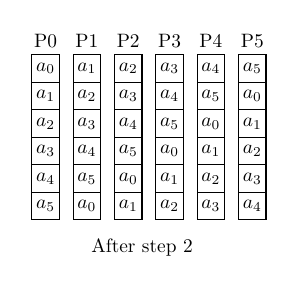
\begin{tikzpicture}[scale=0.35, every node/.style={transform shape}]
	
	%//starting at (0,0)
	
	\draw (0,0) -- (0,6) -- (1,6) -- (1,0) -- cycle;
	\foreach \x in {0,1,2,3,4, 5, 6}
	\draw (0,\x) -- (1,\x);
	
	\foreach \x/\val in {0/$a_5$,1/$a_4$,2/$a_3$,3/$a_2$,4/$a_1$, 5/$a_0$}
	\node [scale=2] at (0.5, 0.5 + \x) {\val};
	
	\foreach \x in {0,1,2,3,4, 5}
	\node [scale=2] at (1.5*\x+0.5 , 6.5) {P\x};
	
	\def\xstep{1.5}
	
	\draw (\xstep+0,0) -- (\xstep+0,6) -- (\xstep+1,6) -- (\xstep+1,0) -- cycle;
	\foreach \x in {0,1,2,3,4, 5, 6}
	\draw (\xstep+0,\x) -- (\xstep+1,\x);
	
	\foreach \x/\val in {0/$a_0$,1/$a_5$,2/$a_4$,3/$a_3$,4/$a_2$, 5/$a_1$}
	\node [scale=2] at (\xstep+0.5, 0.5 + \x) {\val};
	
	\def\xstep{3}
	
	\draw (\xstep+0,0) -- (\xstep+0,6) -- (\xstep+1,6) -- (\xstep+1,0) -- cycle;
	\foreach \x in {0,1,2,3,4, 5, 6}
	\draw (\xstep+0,\x) -- (\xstep+1,\x);
	
	\foreach \x/\val in {0/$a_1$,1/$a_0$,2/$a_5$,3/$a_4$,4/$a_3$, 5/$a_2$}
	\node [scale=2] at (\xstep+0.5, 0.5 + \x) {\val};
	
	
	\def\xstep{4.5}
	
	\draw (\xstep+0,0) -- (\xstep+0,6) -- (\xstep+1,6) -- (\xstep+1,0) -- cycle;
	\foreach \x in {0,1,2,3,4, 5, 6}
	\draw (\xstep+0,\x) -- (\xstep+1,\x);
	
	\foreach \x/\val in {0/$a_2$,1/$a_1$,2/$a_0$,3/$a_5$,4/$a_4$, 5/$a_3$}
	\node [scale=2] at (\xstep+0.5, 0.5 + \x) {\val};
	
	\def\xstep{6}
	
	\draw (\xstep+0,0) -- (\xstep+0,6) -- (\xstep+1,6) -- (\xstep+1,0) -- cycle;
	\foreach \x in {0,1,2,3,4, 5, 6}
	\draw (\xstep+0,\x) -- (\xstep+1,\x);
	
	\foreach \x/\val in {0/$a_3$,1/$a_2$,2/$a_1$,3/$a_0$,4/$a_5$, 5/$a_4$}
	\node [scale=2] at (\xstep+0.5, 0.5 + \x) {\val};
	
	\def\xstep{7.5}
	
	\draw (\xstep+0,0) -- (\xstep+0,6) -- (\xstep+1,6) -- (\xstep+1,0) -- cycle;
	\foreach \x in {0,1,2,3,4, 5, 6}
	\draw (\xstep+0,\x) -- (\xstep+1,\x);
	
	\foreach \x/\val in {0/$a_4$,1/$a_3$,2/$a_2$,3/$a_1$,4/$a_0$, 5/$a_5$}
	\node [scale=2] at (\xstep+0.5, 0.5 + \x) {\val};
	
	\node [scale=2] at (4, -1) {$\textnormal{After step $2$}$};
	\end{tikzpicture}
\end{minipage}
\begin{minipage}{0.3\linewidth}
	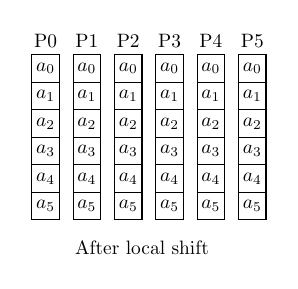
\begin{tikzpicture}[scale=0.35, every node/.style={transform shape}]
	
	%//starting at (0,0)
	
	\draw (0,0) -- (0,6) -- (1,6) -- (1,0) -- cycle;
	\foreach \x in {0,1,2,3,4, 5, 6}
	\draw (0,\x) -- (1,\x);
	
	\foreach \x/\val in {0/$a_5$,1/$a_4$,2/$a_3$,3/$a_2$,4/$a_1$, 5/$a_0$}
	\node [scale=2] at (0.5, 0.5 + \x) {\val};
	
	\foreach \x in {0,1,2,3,4, 5}
	\node [scale=2] at (1.5*\x+0.5 , 6.5) {P\x};
	
	\def\xstep{1.5}
	
	\draw (\xstep+0,0) -- (\xstep+0,6) -- (\xstep+1,6) -- (\xstep+1,0) -- cycle;
	\foreach \x in {0,1,2,3,4, 5, 6}
	\draw (\xstep+0,\x) -- (\xstep+1,\x);
	
	\foreach \x/\val in {0/$a_5$,1/$a_4$,2/$a_3$,3/$a_2$,4/$a_1$, 5/$a_0$}
	\node [scale=2] at (\xstep+0.5, 0.5 + \x) {\val};
	
	\def\xstep{3}
	
	\draw (\xstep+0,0) -- (\xstep+0,6) -- (\xstep+1,6) -- (\xstep+1,0) -- cycle;
	\foreach \x in {0,1,2,3,4, 5, 6}
	\draw (\xstep+0,\x) -- (\xstep+1,\x);
	
	\foreach \x/\val in {0/$a_5$,1/$a_4$,2/$a_3$,3/$a_2$,4/$a_1$, 5/$a_0$}
	\node [scale=2] at (\xstep+0.5, 0.5 + \x) {\val};
	
	
	\def\xstep{4.5}
	
	\draw (\xstep+0,0) -- (\xstep+0,6) -- (\xstep+1,6) -- (\xstep+1,0) -- cycle;
	\foreach \x in {0,1,2,3,4, 5, 6}
	\draw (\xstep+0,\x) -- (\xstep+1,\x);
	
	\foreach \x/\val in {0/$a_5$,1/$a_4$,2/$a_3$,3/$a_2$,4/$a_1$, 5/$a_0$}
	\node [scale=2] at (\xstep+0.5, 0.5 + \x) {\val};
	
	\def\xstep{6}
	
	\draw (\xstep+0,0) -- (\xstep+0,6) -- (\xstep+1,6) -- (\xstep+1,0) -- cycle;
	\foreach \x in {0,1,2,3,4, 5, 6}
	\draw (\xstep+0,\x) -- (\xstep+1,\x);
	
	\foreach \x/\val in {0/$a_5$,1/$a_4$,2/$a_3$,3/$a_2$,4/$a_1$, 5/$a_0$}
	\node [scale=2] at (\xstep+0.5, 0.5 + \x) {\val};
	
	\def\xstep{7.5}
	
	\draw (\xstep+0,0) -- (\xstep+0,6) -- (\xstep+1,6) -- (\xstep+1,0) -- cycle;
	\foreach \x in {0,1,2,3,4, 5, 6}
	\draw (\xstep+0,\x) -- (\xstep+1,\x);
	
	\foreach \x/\val in {0/$a_5$,1/$a_4$,2/$a_3$,3/$a_2$,4/$a_1$, 5/$a_0$}
	\node [scale=2] at (\xstep+0.5, 0.5 + \x) {\val};
	
	\node [scale=2] at (4, -1) {$\textnormal{After local shift}$};
	\end{tikzpicture}
\end{minipage}
\end{frame}

\end{document} 